\appendix
\chapter{Appendix - Character Animations}
\section{Emotes}

\begin{figure}[H]
\centering
  \caption{List of emotes}
  \label{fig:emotes_list}
  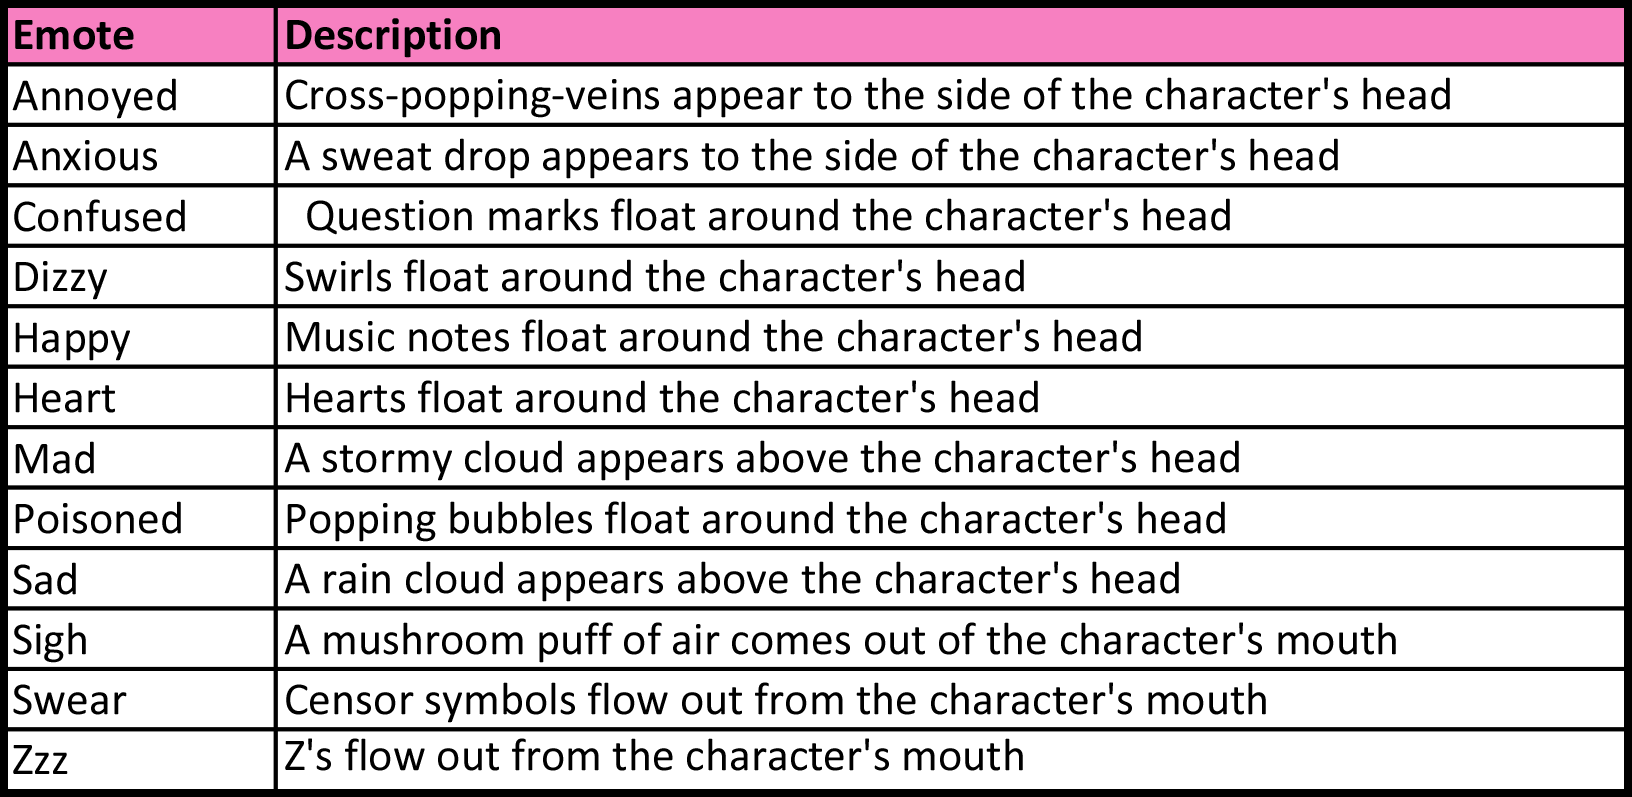
\includegraphics[width=0.95\textwidth, height=0.7\paperheight, keepaspectratio=true]{images/table_emotes}
\end{figure}

\clearpage
\section{Skeletal Animations}

\begin{figure}[H]
\centering
  \caption{List of Skeletal Animations}
  \label{fig:animations_list}
  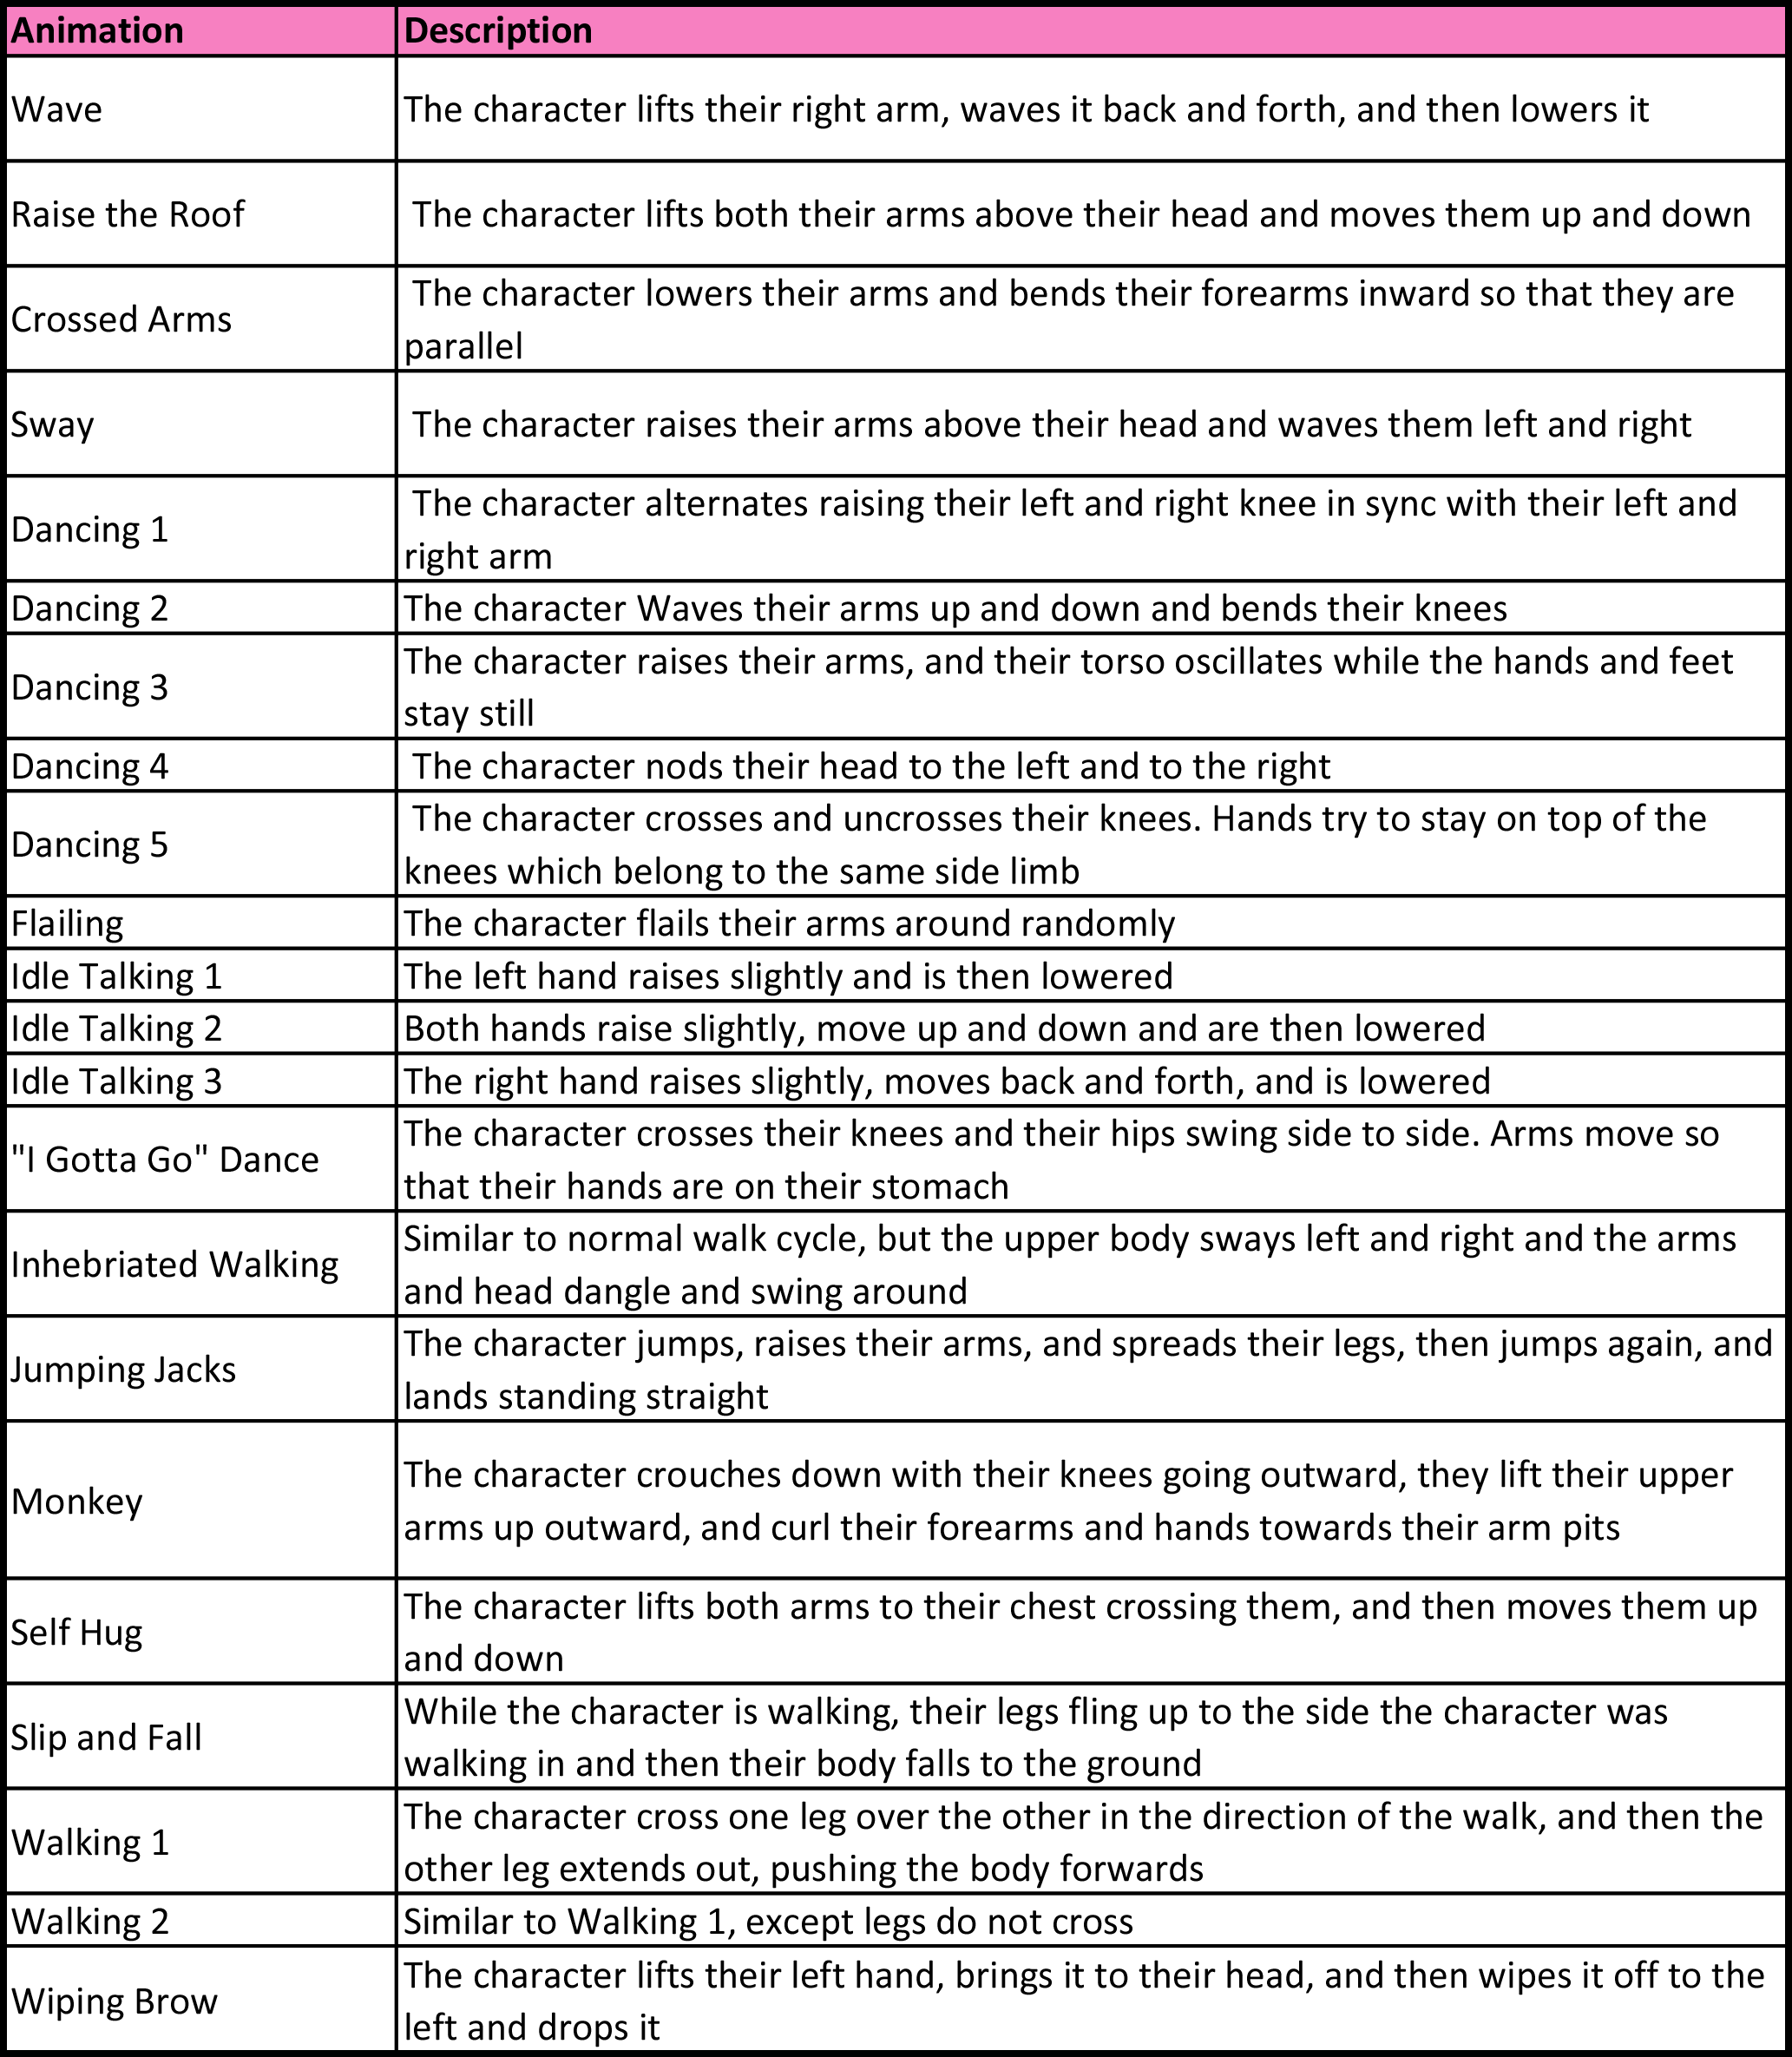
\includegraphics[width=0.95\textwidth, height=0.7\paperheight, keepaspectratio=true]{images/table_animations}
\end{figure}

\chapter{Appendix - Audio Assets}
\section{Sound Effects}

\begin{figure}[H]
\centering
  \caption{List of sound effects}
  \label{fig:sound_effects_list}
  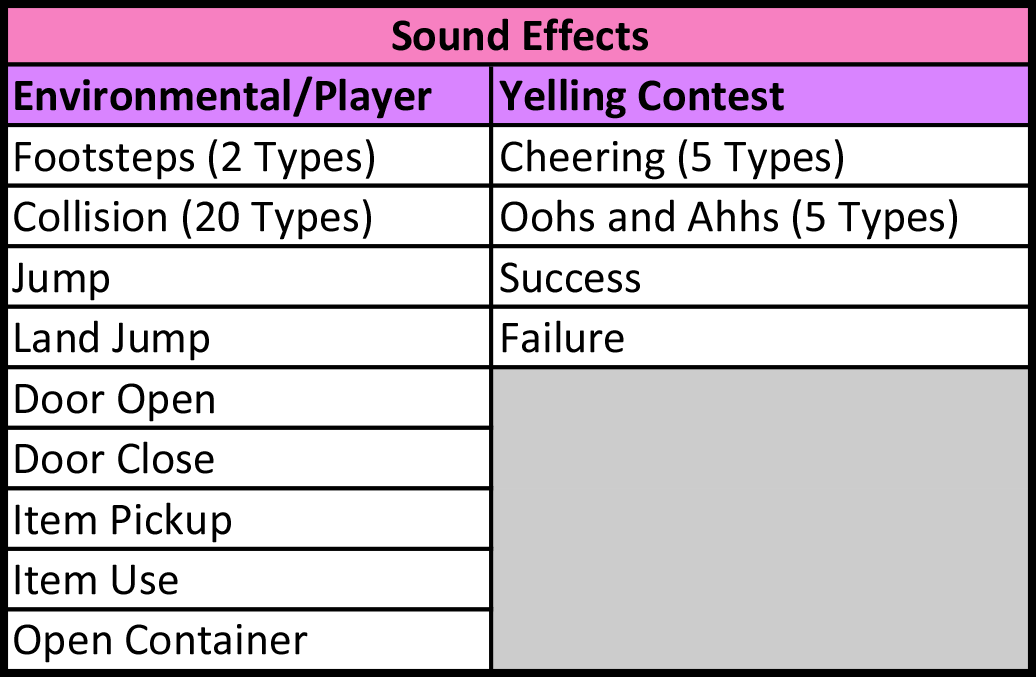
\includegraphics[width=0.95\textwidth, height=0.5\paperheight, keepaspectratio=true]{images/table_sound_effects}
\end{figure}

\clearpage
\chapter{Appendix - Environment Assets}
\section{List of Furniture Objects}

\begin{figure}[H]
\centering
  \caption{List of furniture objects and the components they will be comprised of}
  \label{fig:furniture_list}
  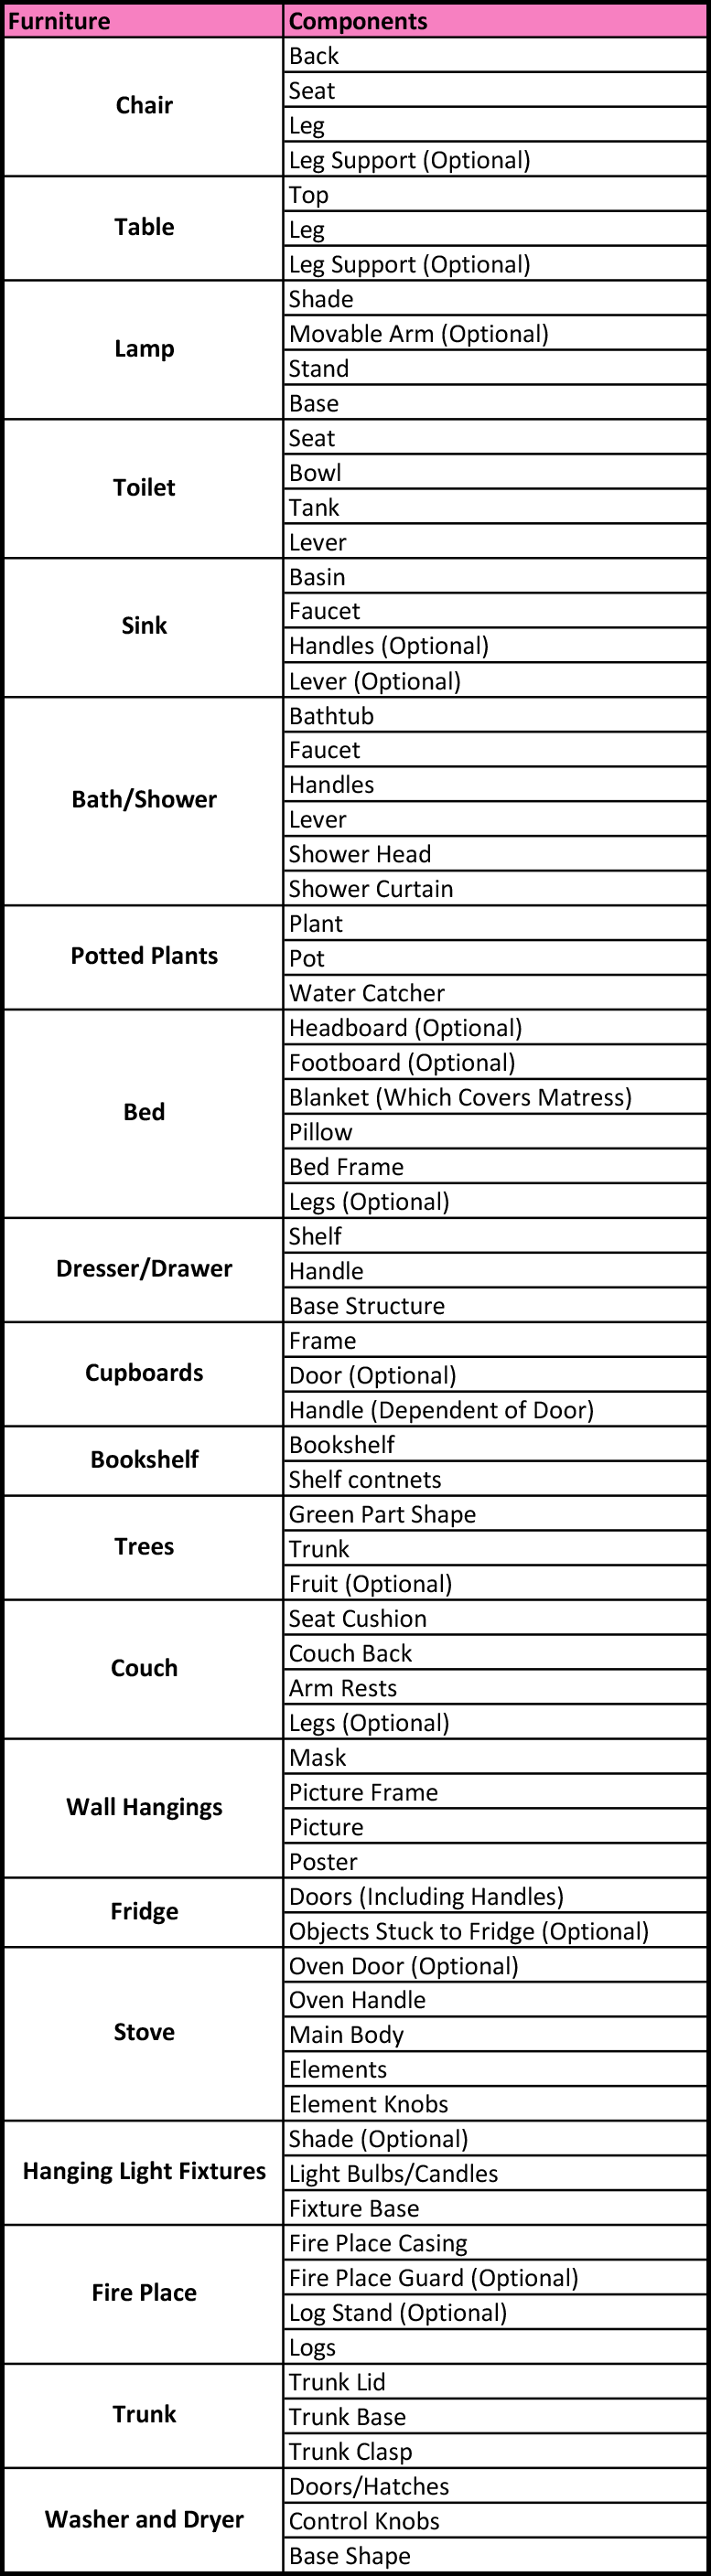
\includegraphics[width=0.95\textwidth, height=0.5\paperheight, keepaspectratio=true]{images/table_furniture}
  
\end{figure}


\clearpage
\section{List of Props}

\begin{figure}[H]
\centering
  \caption{List of 3D props and their respective masses}
  \label{fig:props_list}
  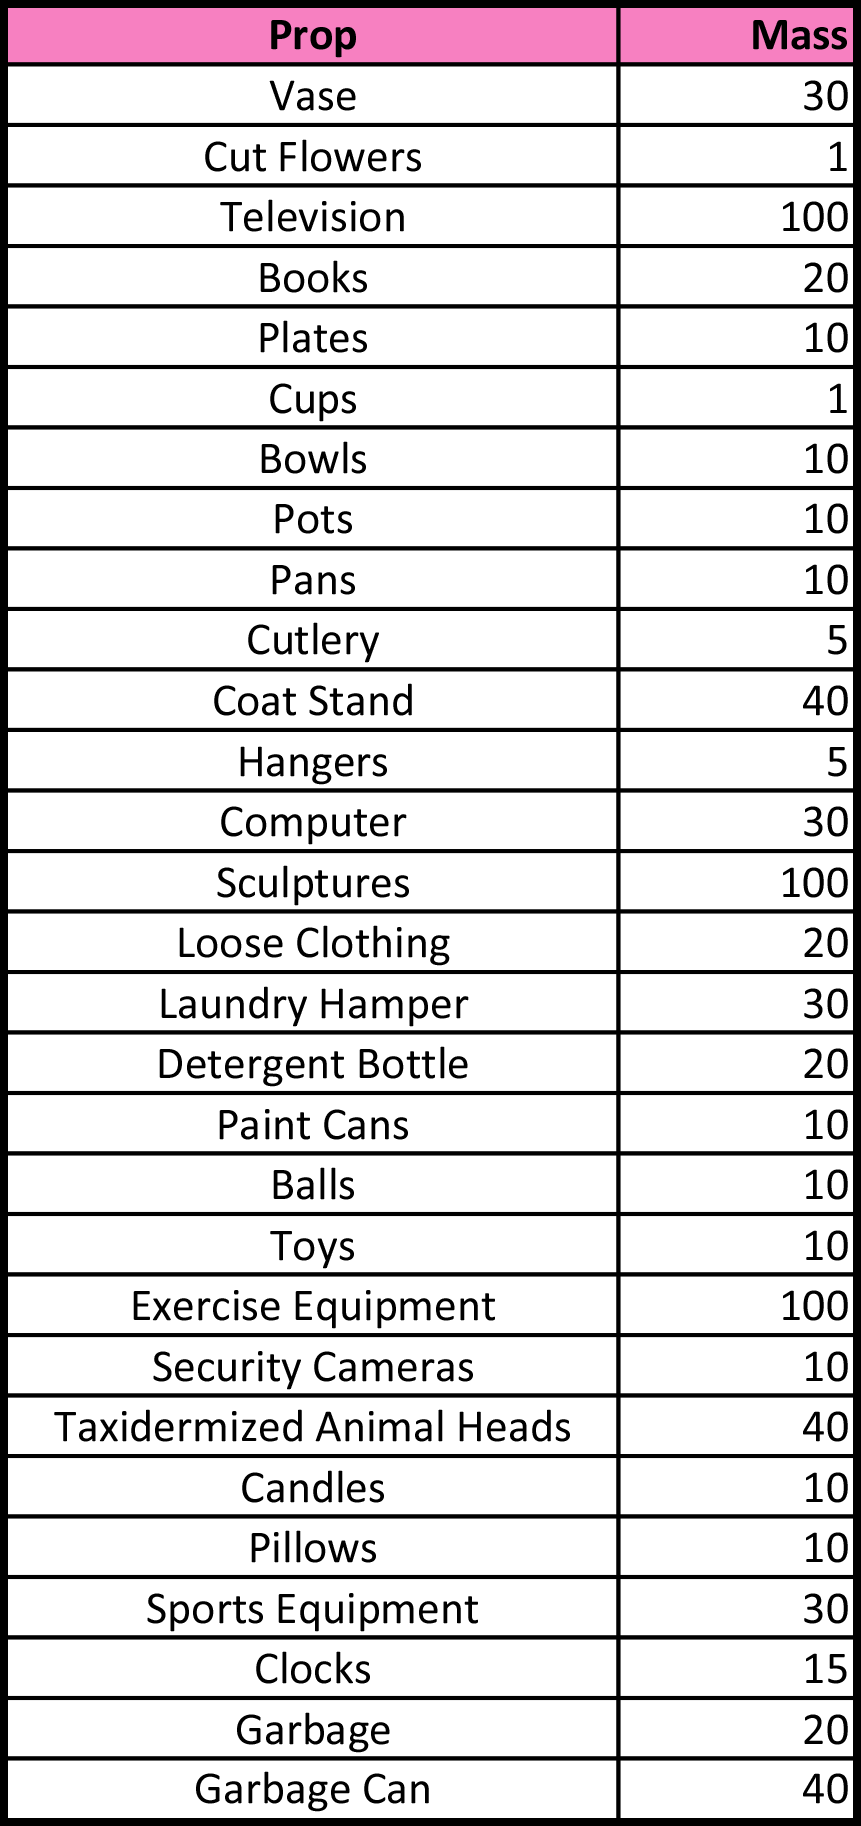
\includegraphics[width=0.95\textwidth, height=0.5\paperheight, keepaspectratio=true]{images/table_3D_props}
\end{figure}

\clearpage
\section{Interactive Items}
\begin{figure}[H]
	\centering
\includegraphics[width=.75\linewidth, height=0.8\paperheight, keepaspectratio=true]{images/items_banana}
	\caption{Banana - perishable food item}
\end{figure}
\begin{figure}[p]
	\centering
\includegraphics[height=.8\paperheight]{images/items_bottledsoftdrink}
	\caption{Bottled Soft-Drink - perishable food item}
\end{figure}
\begin{figure}[p]
	\centering
\includegraphics[width=.8\linewidth]{images/items_carrot}
	\caption{Carrot - perishable food item}
\end{figure}
\begin{figure}[p]
	\centering
\includegraphics[width=.8\linewidth, height=.8\paperheight, keepaspectratio=true]{images/items_cupcake}
	\caption{Cupcake - perishable food item}
\end{figure}
\begin{figure}[p]
	\centering
\includegraphics[width=.8\linewidth]{images/items_donut}
	\caption{Doughnut - perishable food item}
\end{figure}
\begin{figure}[p]
	\centering
\includegraphics[height=.8\paperheight]{images/items_icecreamcone}
	\caption{Ice Cream Cone - perishable food item}
\end{figure}
\begin{figure}[p]
	\centering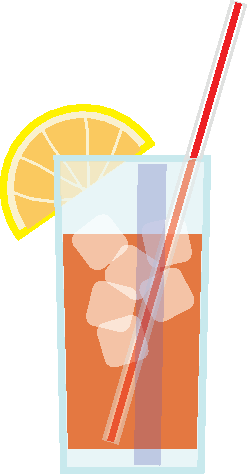
\includegraphics[height=.8\paperheight]{images/items_iceddrink}
	\caption{Iced Beverage - perishable food item}
\end{figure}
\begin{figure}[p]
	\centering
\includegraphics[height=.8\paperheight]{images/items_key}
	\caption{Key - non-consumable item}
\end{figure}
\begin{figure}[p]
	\centering
\includegraphics[height=.8\paperheight]{images/items_lightswitch}
	\caption{Light Switch - uncollectable item}
\end{figure}
\begin{figure}[p]
	\centering
\includegraphics[height=.8\paperheight]{images/items_milk}
	\caption{Milk - perishable food item}
\end{figure}
\begin{figure}[p]
	\centering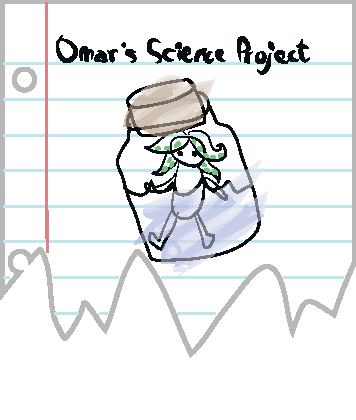
\includegraphics[height=.8\paperheight]{images/items_note}
	\caption{Omar's Old School Assignment - non-consumable item}
\end{figure}
\begin{figure}[p]
	\centering
\includegraphics[height=.8\paperheight]{images/items_popsicle}
	\caption{Popsicle - perishable food item}
\end{figure}
\begin{figure}[p]
	\centering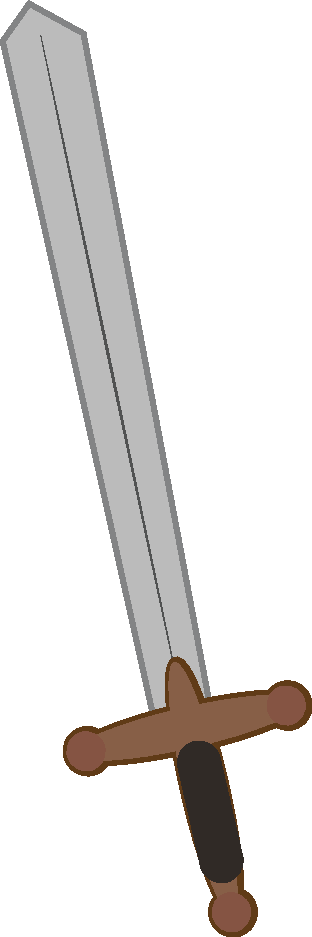
\includegraphics[height=.8\paperheight]{images/items_sword}
	\caption{Sword - non-consumable item}
\end{figure}

\clearpage
\section{Game Flow}
Flowchart of main gameplay loops.

\subsection{Yelling Contest}
\begin{figure}[H]
\centering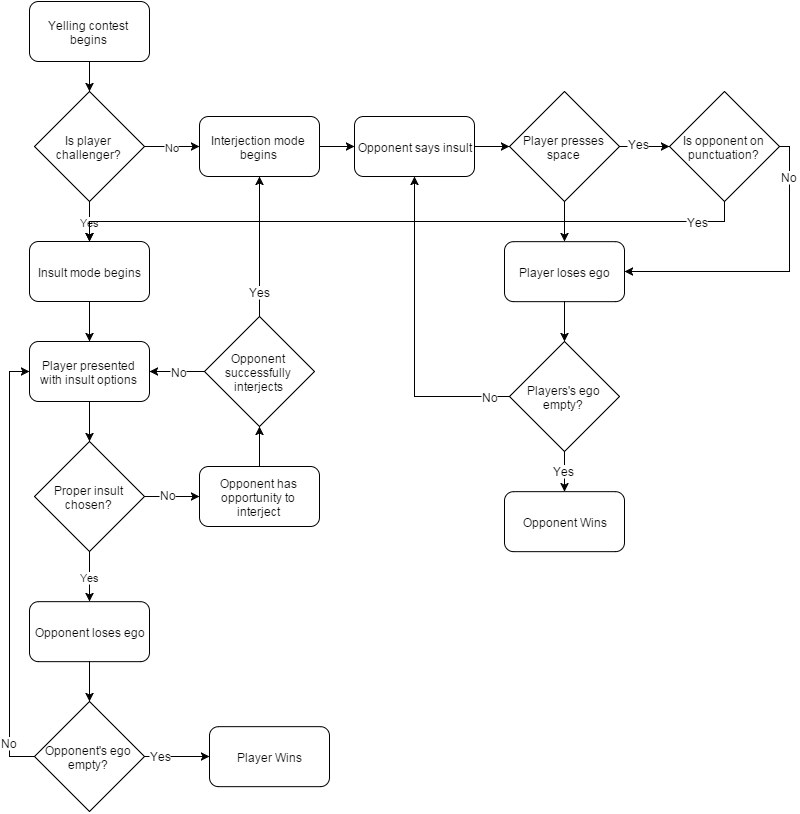
\includegraphics[width=0.5\textwidth, height=0.8\paperheight, keepaspectratio=true]{images/YellingContest}
  \caption{Yelling Contest Flow}
  \label{fig:flow_yelling_contest}
\end{figure}

\subsection{Conversation}
\begin{figure}[H]
\centering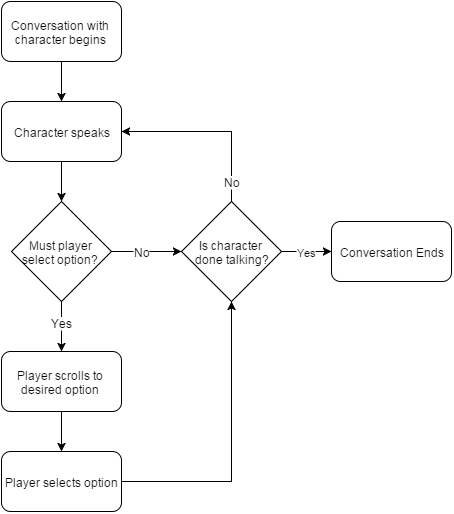
\includegraphics[width=0.5\textwidth, height=0.8\paperheight, keepaspectratio=true]{images/Conversation}
  \caption{Conversation Flow}
  \label{fig:flow_conversation}
\end{figure}

\subsection{Main Menu}
\begin{figure}[H]
\centering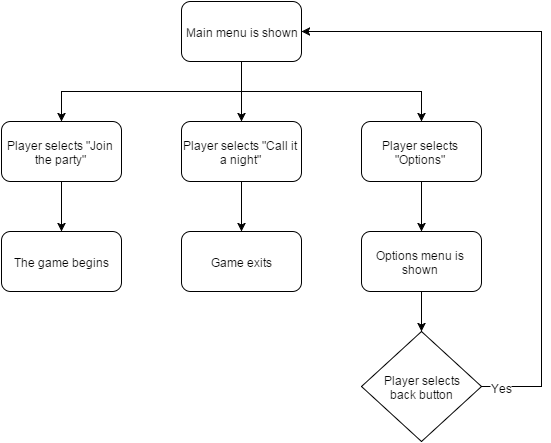
\includegraphics[width=0.5\textwidth, height=0.8\paperheight, keepaspectratio=true]{images/MainMenu}
  \caption{Main Menu Flow}
  \label{fig:flow_scenario}
\end{figure}

\clearpage

\subsection{Scenario}
\begin{figure}[H]
\centering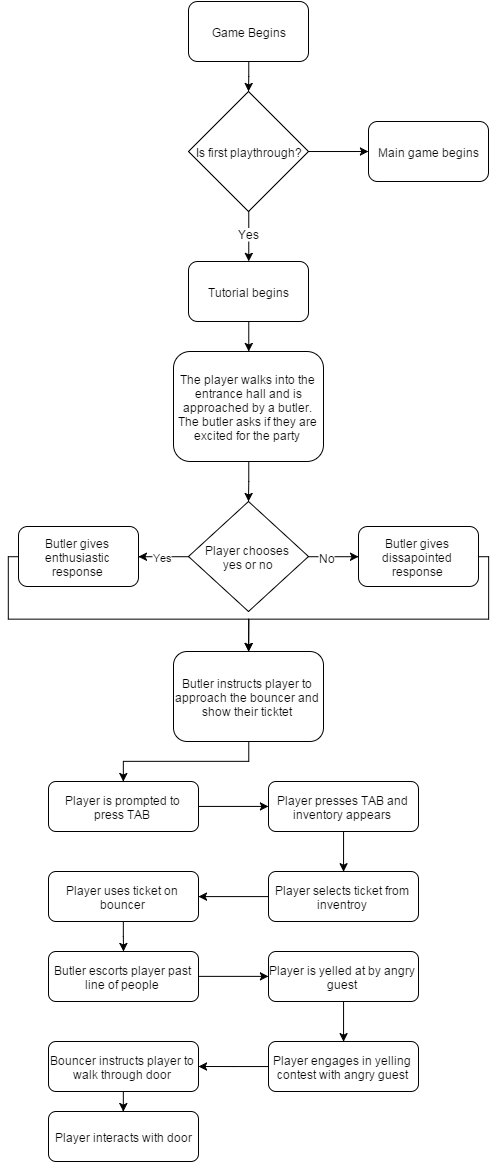
\includegraphics[width=0.5\textwidth, height=0.8\paperheight, keepaspectratio=true]{images/Tutorial}
  \caption{Tutorial}
  \label{fig:flow_tutorial}
\end{figure}

\subsection{Recruiting Character}
\begin{figure}[H]
\centering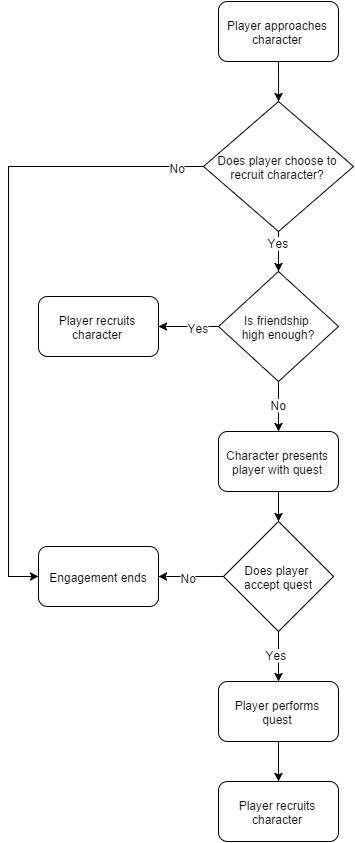
\includegraphics[width=0.5\textwidth, height=0.8\paperheight, keepaspectratio=true]{images/Recruit}
  \caption{Recruiting Characters}
  \label{fig:flow_recruit}
\end{figure}

\subsection{Item Discovery and Use}
\begin{figure}[H]
\centering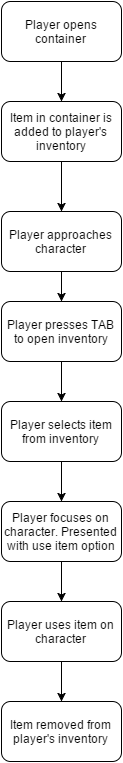
\includegraphics[width=0.5\textwidth, height=0.8\paperheight, keepaspectratio=true]{images/ItemUse}
  \caption{Item Discovery and Use}
  \label{fig:flow_item}
\end{figure}

\subsection{Scenario Creation and Use}
\begin{figure}[H]
\centering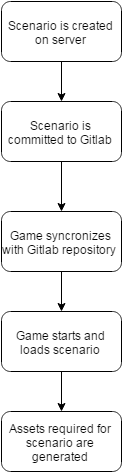
\includegraphics[width=0.5\textwidth, height=0.8\paperheight, keepaspectratio=true]{images/ScenarioLoading}
  \caption{Scenario Creation and Use}
  \label{fig:flow_scenario_loading}
\end{figure}


\clearpage
\section{Room Generation}
Flowcharts of room generation procedures.

\subsection{House Generation}
\begin{figure}[H]
\centering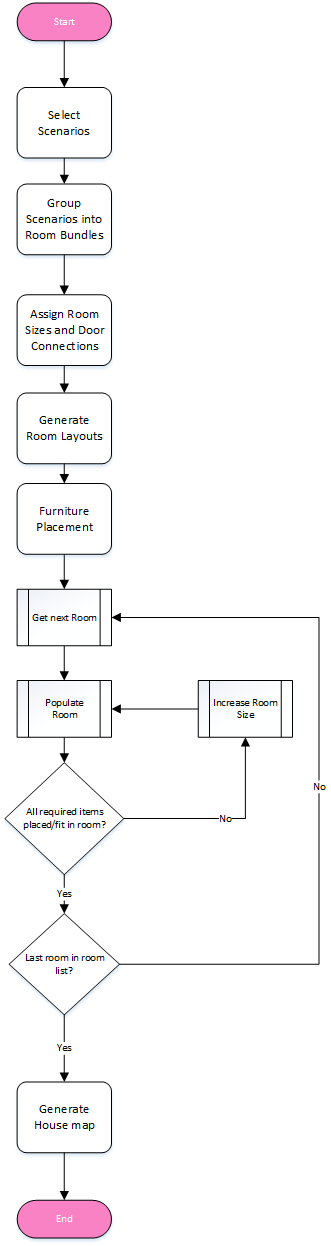
\includegraphics[width=0.95\linewidth, height=0.7\paperheight, keepaspectratio=true]{images/RoomGeneration_HouseGeneration_Flowchart}
  \caption{House Generation Flow}
  \label{fig:flow_house_generation}
\end{figure}

\clearpage
\subsection{Furniture Placement}
\begin{figure}[H]
\centering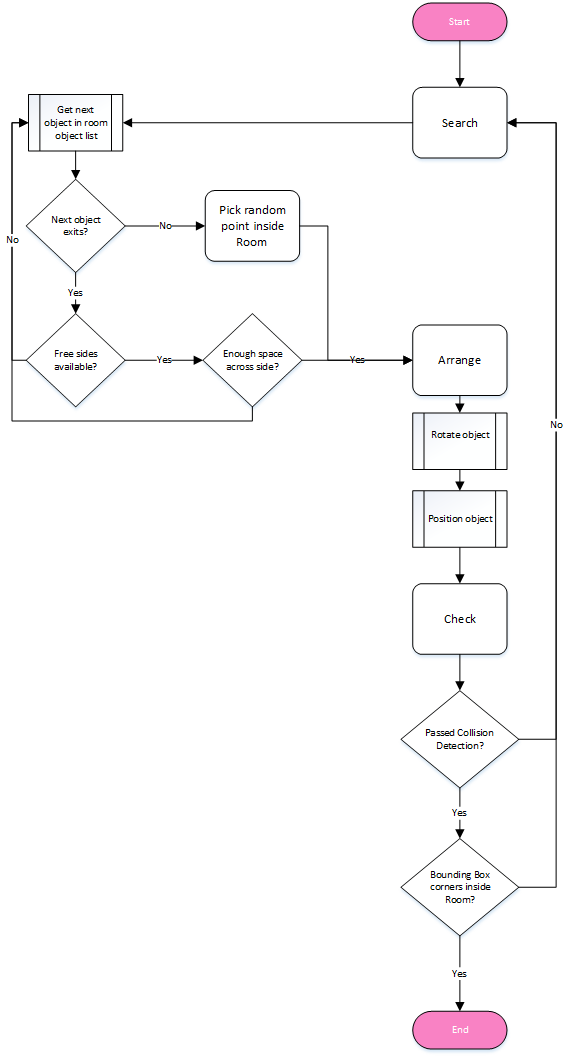
\includegraphics[width=0.95\linewidth, height=0.7\paperheight, keepaspectratio=true]{images/RoomGeneration_FurniturePlacement_Flowchart}
  \caption{Furniture Placement Flow}
  \label{fig:flow_furniture_placement}
\end{figure}

\chapter{Appendix - Scenario Editor Mockups}
\label{app:mockups}
Mockups of certain planned views for the Scenario Editor application.

\section{Regular view (Character)}

\begin{figure}[H]
\centering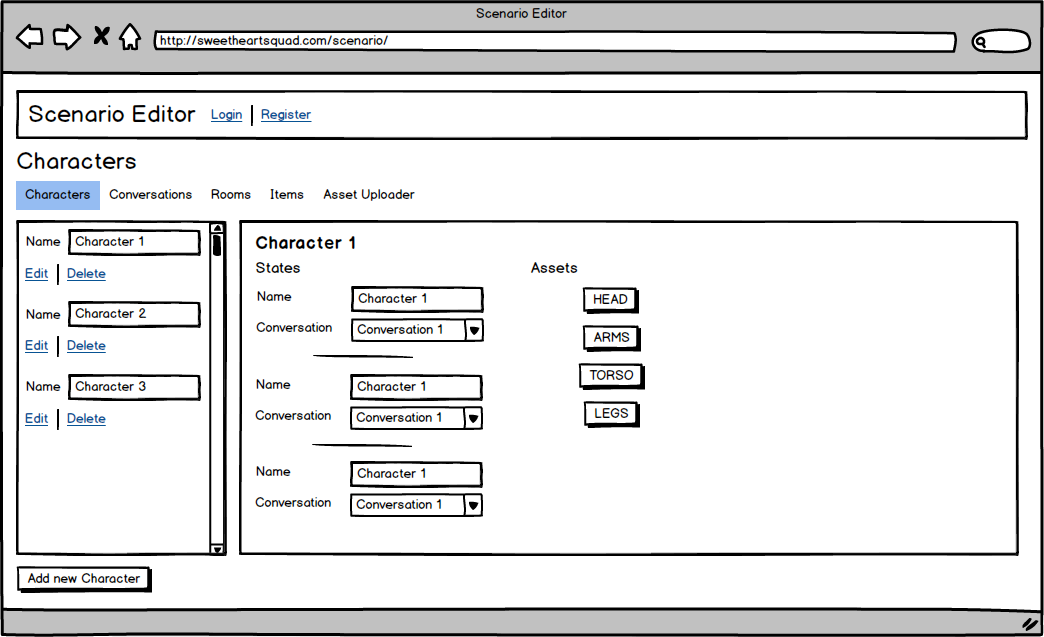
\includegraphics[width=0.95\linewidth, height=0.7\paperheight, keepaspectratio=true]{images/Character1}
  \caption{The character view.}
  \label{fig:mockup_char_1}
\end{figure}

\begin{figure}[p]
\centering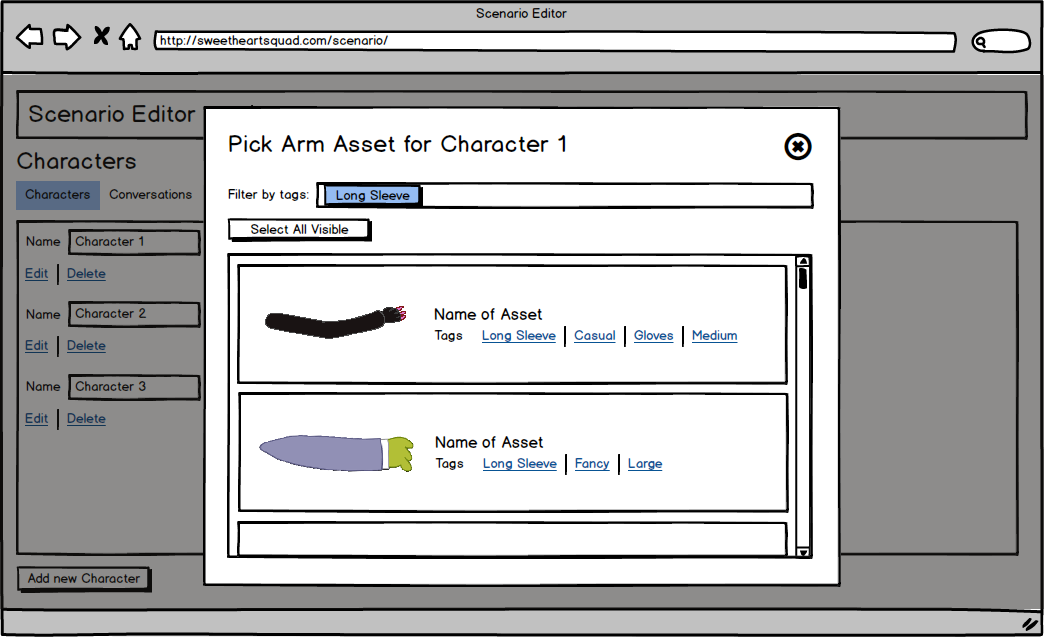
\includegraphics[width=0.95\linewidth, height=0.7\paperheight, keepaspectratio=true]{images/Character2}
  \caption{Asset selection view. User can select one or more possible components for a character's arm.}
  \label{fig:mockup_char_2}
\end{figure}

\begin{figure}[p]
\centering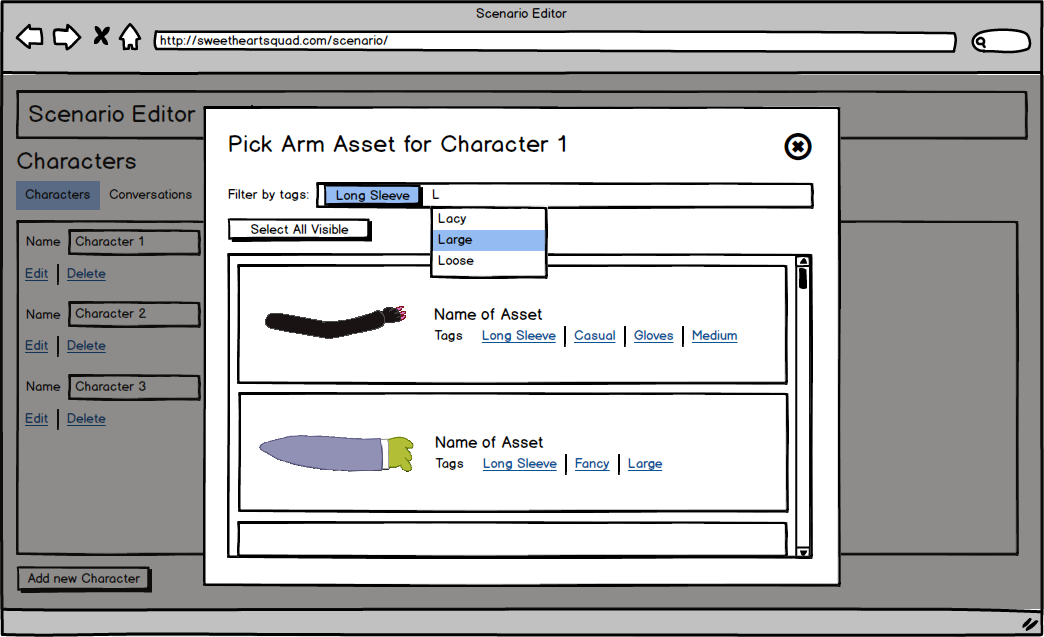
\includegraphics[width=0.95\linewidth, height=0.7\paperheight, keepaspectratio=true]{images/Character3}
  \caption{Asset selection view. User can search for components by tag.}
  \label{fig:mockup_char_3}
\end{figure}

\begin{figure}[p]
\centering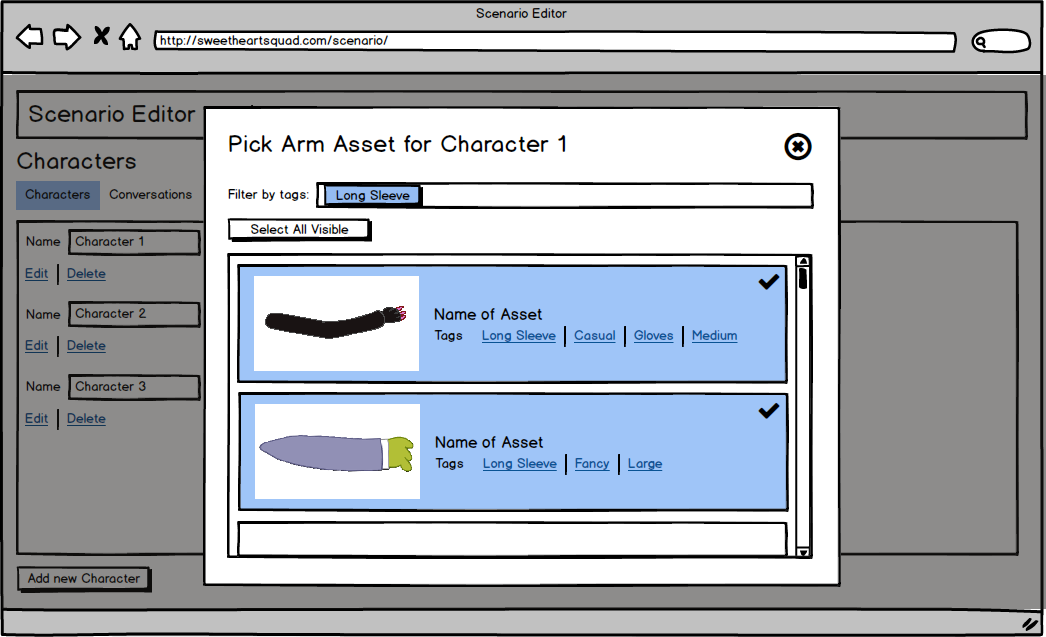
\includegraphics[width=0.95\linewidth, height=0.7\paperheight, keepaspectratio=true]{images/Character4}
  \caption{Asset selection view. User has chosen two possible components for this character. One will be randomly selected whenever this scenario is loaded into \ourgame{}.}
  \label{fig:mockup_char_4}
\end{figure}

\clearpage
\section{Asset Uploader view}

\begin{figure}[H]
\centering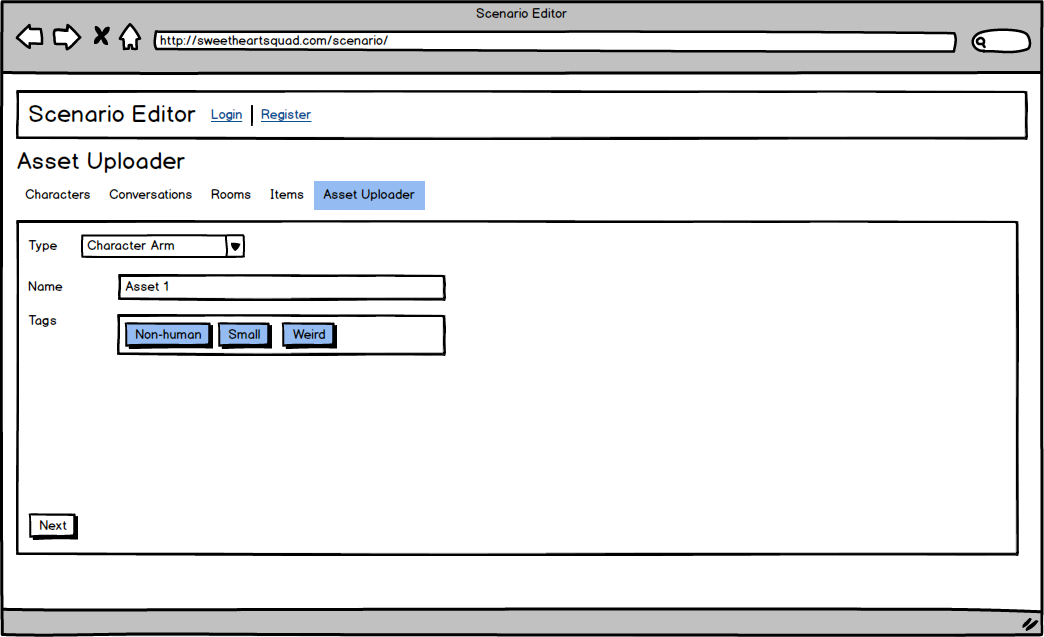
\includegraphics[width=0.95\linewidth, height=0.7\paperheight, keepaspectratio=true]{images/AssetUploader_Arm1}
  \caption{The first Asset Uploader screen. The user can specify what type of asset is being uploaded. (In this case, a "character arm" asset.)}
  \label{fig:mockup_asset_1}
\end{figure}

\begin{figure}[p]
\centering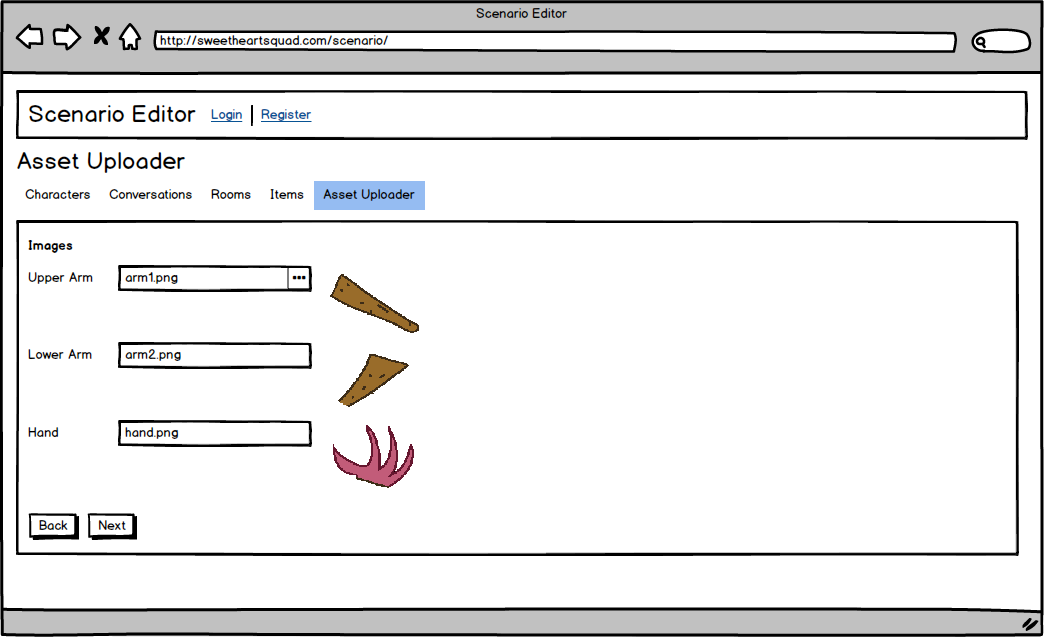
\includegraphics[width=0.95\linewidth, height=0.7\paperheight, keepaspectratio=true]{images/AssetUploader_Arm2}
  \caption{The second screen of the Asset Uploader. The user uploads the required images for this asset.}
  \label{fig:mockup_asset_2}
\end{figure}

\begin{figure}[p]
\centering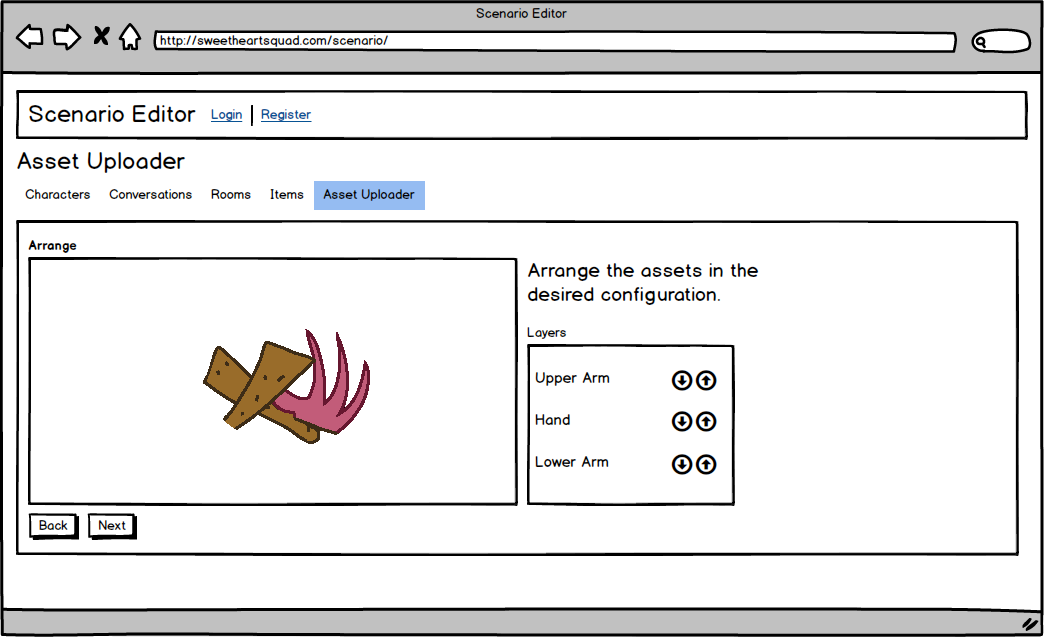
\includegraphics[width=0.95\linewidth, height=0.7\paperheight, keepaspectratio=true]{images/AssetUploader_Arm3}
  \caption{The third screen of the Asset Uploader. The user arranges the images as they will appear in the game world.}
  \label{fig:mockup_asset_3}
\end{figure}

\begin{figure}[p]
\centering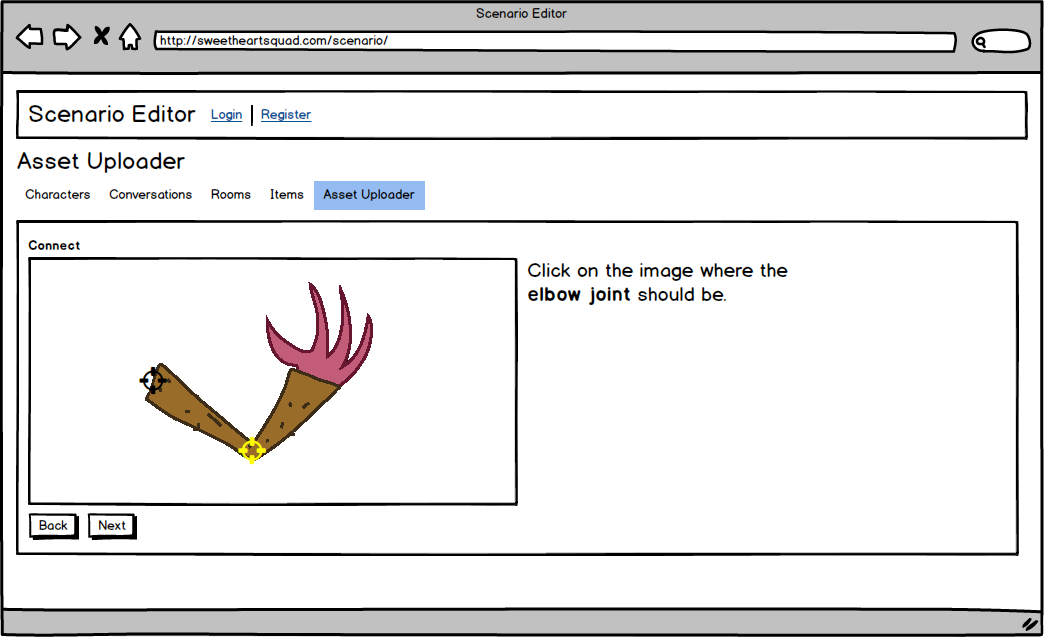
\includegraphics[width=0.95\linewidth, height=0.7\paperheight, keepaspectratio=true]{images/AssetUploader_Arm4}
  \caption{The fourth screen of the Asset Uploader. The user specifies the joints that will connect the images together.}
  \label{fig:mockup_asset_4}
\end{figure}

\begin{figure}[H]
\centering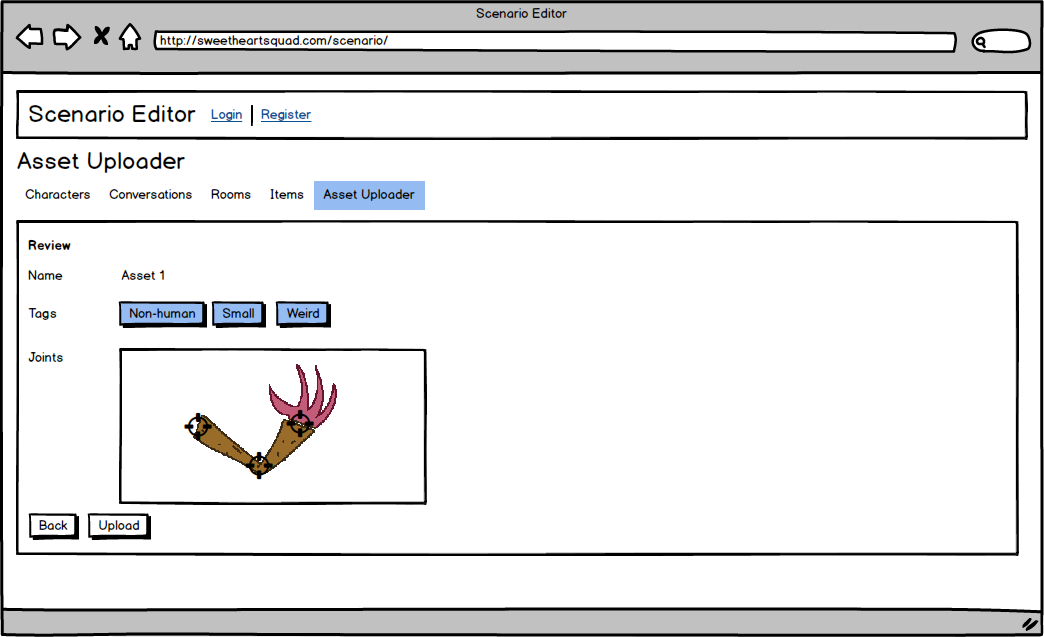
\includegraphics[width=0.95\linewidth, height=0.7\paperheight, keepaspectratio=true]{images/AssetUploader_Arm5}
  \caption{The final screen of the Asset Uploader. The user can review their work, go back to previous screens, or upload the finished asset to the server.}
  \label{fig:mockup_asset_5}
\end{figure}


\chapter{Appendix - Scenario Data Model}
\label{app:DataModel}
\begin{figure}[H]
\centering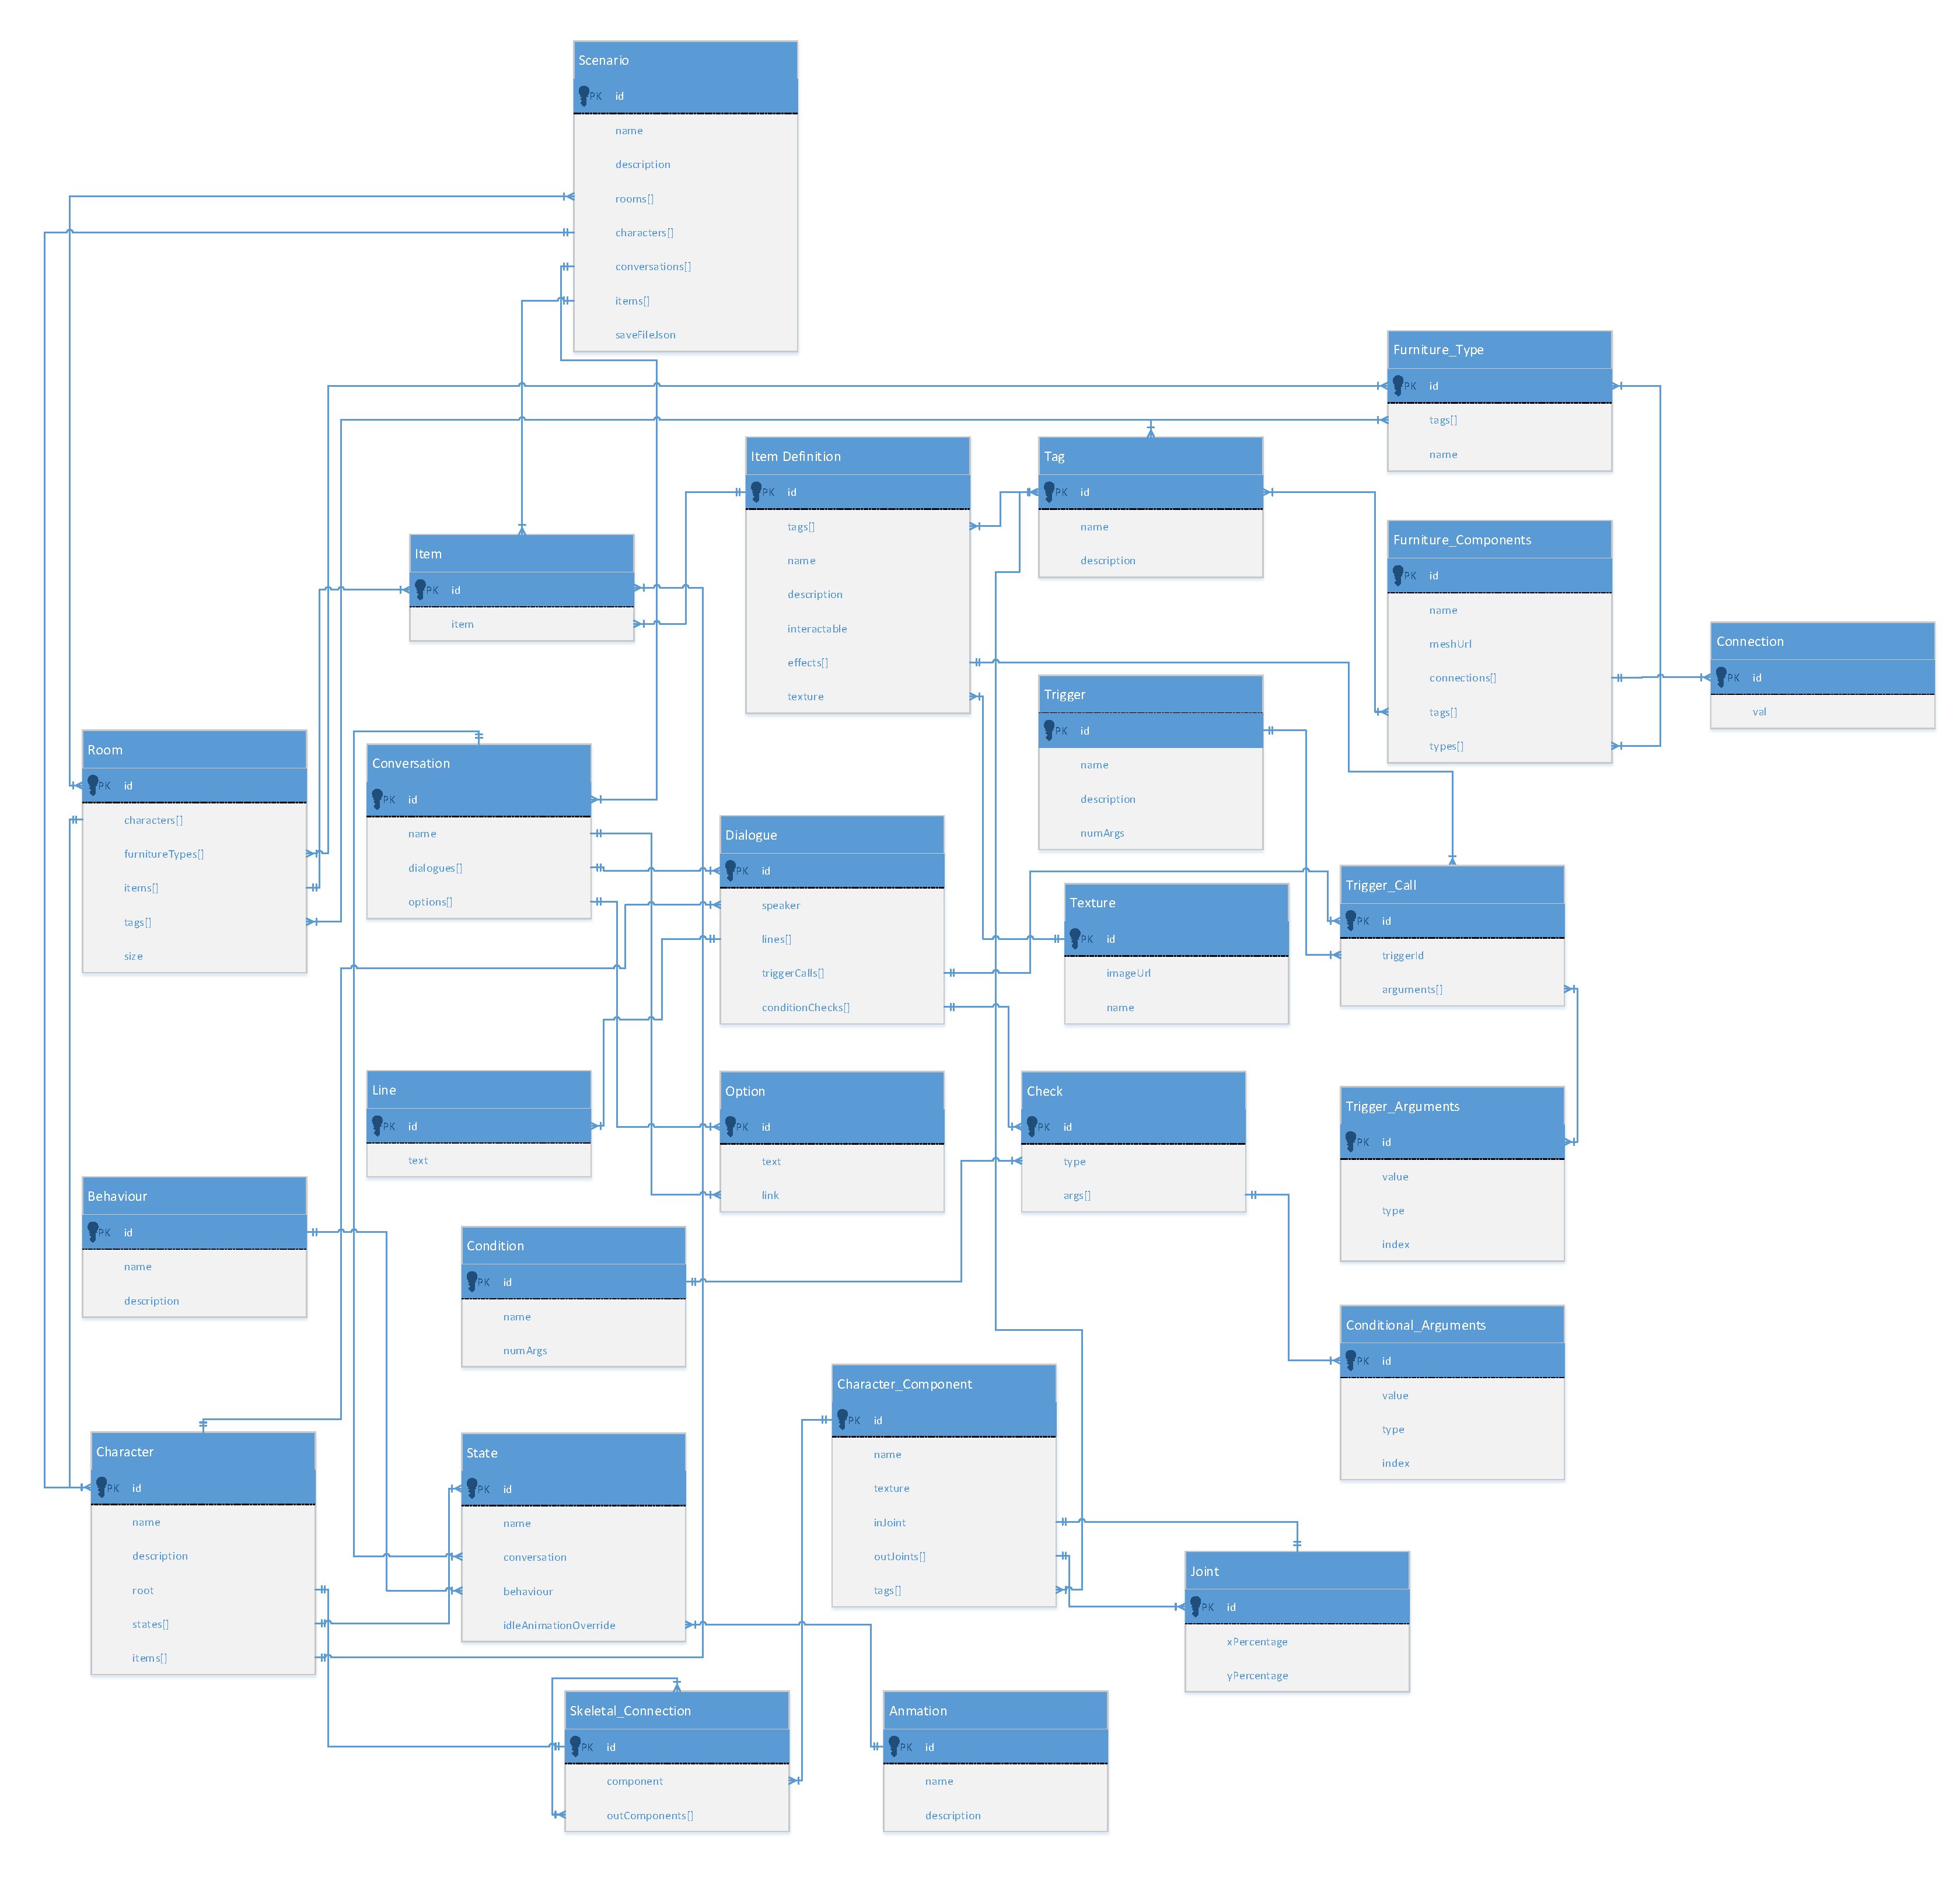
\includegraphics[width=0.95\linewidth, height=0.75\paperheight, keepaspectratio=true]{DataModel}
  \caption{A UML diagram of the data model behind \ourgame{}'s scenarios.}
  \label{fig:UML}
\end{figure}


\chapter{Appendix - Characters}
\label{app:characters}

%\newpage

\character{chara_reed}
{Goodsee Beauregard, P.I.}
{Main Character}
{No-nonsense, Inquisitive, Jittery}
{Beauregard has been investigating the mysterious Omar Clean for her own purposes. When Omar Clean is murdered, she becomes obsessed with solving the murder and figuring out the mystery behind the man. And the man behind the mystery, too.}
{The player will help Beauregard determine the murderer of Omar Clean, by discovering clues and interrogating party guests.}

\character{chara_portrait_omar}
{Omar "The Portrait" Clean}
{Main Character}
{Power-hungry, Devious, Intelligent}
{Omar Clean is a scientist. He discovered a way to explore multiple dimensions and meet other versions of himself that pursued different paths in life. He decides to steal the skills and powers of these alternate versions of himself to become all-powerful. His plan backfires and he steals all the weaknesses of his alternate selves, which ages and damages him. He manages to preserve himself inside a portrait before his body is completely destroyed.}
{He wants the player to fix his machine so he can reverse the damage done to him and allow him to return to his physical form.}

\character{chara_protector_omar}
{Omar "The Protector" Clean}
{Main Character}
{Intelligent, Virtuous}
{The Protector is the version of Omar Clean from the initial universe the player explores. He is a scientist who discovers a way to explore alternate universes. He finds out that another Omar Clean (The Portrait) was trying to harness the power of other versions of Omar Cleans from throughout the multiverse. He ensures that Portrait Omar stays imprisoned and cannot hurt the other Omars.}
{He wants the player to help him keep Portrait Omar imprisoned and protect the portrait. If the portrait gets destroyed, or Portrait Omar is freed, the weaknesses of the other Omar Cleans will be restored. One of these weaknesses is aging, so if the portrait is destroyed it will mean that all versions of Omar Clean will die of old age.}

\character{chara_cool_omar}
{Omar "Getaway" Clean}
{Side Character}
{Suave, Clever, Pragmatic, Dangerous, Handsome, Charming, Devious, and a jack-of-all-trades}
{This version of Omar Clean was once a treasure hunter: breaking hearts, making enemies, and travelling the world in search of ancient artifacts. The years and the injuries caught up to him, and he was forced to settle down. Now he spends his days throwing lavish parties in his immense mansion for his many friends and confidantes. He rarely attends the parties, so as to avoid assassins and jilted exes, but he has been known to appear briefly to steal hearts, and any unattended goods.}
{The player can meet this Omar Clean in a certain alternate universe. Upon finding him, he tells the player that there is a federal agent looking to capture him. The player can then decide to help him escape from the agent, or to leave him to fend for himself. If the player helps Omar escape, he falls in love with the player, and will attempt to get the player to stay with him.}

\character{chara_robo_omar}
{Omar "Waffle Iron" Clean}
{Side Character}
{Curious, Awkward}
{This version of Omar Clean was once an ordinary man, who lived an ordinary life, and got into an ordinary car accident and died. Many decades later, an unknown  scientist dug Omar out of an ordinary cemetery and used his ordinary brain to grant sentience to a robotic waffle iron. This waffle iron Omar Clean desired to become human again, but didn't know how to integrate back into human society. He began to throw large parties in an attempt to study human behaviour.}
{The player can meet this Omar Clean in a certain alternate universe. The player can talk to Omar Clean and learn the true nature of his parties. The player can attempt to convince Omar to stop his research, or agree to answer Omar's questions to aid his re-integration.}

\character{chara_Crash}
{Crash}
{Side Character}
{Tired}
{Crash is a member of a local fraternity. He is attending Omar Clean's party with his frat brothers, who believe Omar's mansion to be a new frat house.}
{Crash is a very tired duck. He is leaning against a door, sleeping. To gain access to the door, the player must go to a nearby kitchen and find a cup of coffee to wake Crash up.}

\character{chara_JonJon}
{Jon-Jon}
{Side Character}
{Loud, Intoxicated, Likes to Joke Around, Loves to Party}
{Jon-Jon is an old sailor turned smuggler that enjoys a good hefty drink now and again. He met Omar Clean while he was working off the northern coast, helping him acquire some special goods. After some close calls they became close friends. Though while he was originally just there to enjoy the party, old habits die hard, and Jon-Jon is now smuggling contraband into the party.}
{The player can find Jon-Jon, drunkenly dancing in the middle of the living room. He'll request the player to have a few drinks with him. If the player obliges, at the temporary cost of some of their D.I.S.S. stats, he will give you some powerful items to heal your \textbf{Voice} attributes. As a loud man himself, Jon-Jon is empathetic to your struggles.}

\character{chara_Wilson}
{Wilson}
{Side Character}
{He likes to rap, he don't take crap, if you talk about his momma he'll give you a slap. He likes to dance, its his one romance, if you wanna tango you won't stand a chance. He likes to diss, you won't be missed, if you really sad after he'll give you a kiss.}
{Wilson is a rowdy boy that came to the party with his crew. Unfortunately they've been causing trouble, bullying other party patrons.}
{Wilson decides to pick a fight with the player. Defeat him and gain the respect of many party people!}

\character{chara_Alphonse}
{Alphonse}
{Side Character}
{Paranoid, On Edge, Spaced Out}
{He came with his rowdy gang of friends led by Wilson in the hopes of having a crazy time.}
{Alphonse can't enjoy the party until he gets his unsalted butter. Unsalted butter gets him rowdy, by golly! The player must find him unsalted butter to appease him. If the player gets him salted butter, he will drag the player into a Yelling contest.}

\character{chara_Jacky-Jam}
{Jacky-Jam}
{Side Character}
{Likes to Beatbox, Not Very Bright, A Follower}
{He is one of Wilson's Crew.}
{He picks a fight with the player, dragging them into a Yelling contest. If the player beats him, he will join their squad.}

\character{chara_dougie}
{Dougie}
{Side Character}
{Good-natured, A real jokester}
{He came to Omar Clean's party to get his prank on!}
{He has come up with an elaborate prank to dump water on his buddy Johnny Q's head. He will ask the player to collect supplies for him and help set them up.}

\character{chara_johnny_q}
{Johnny Q}
{Side Character}
{Goofy, Loud}
{He just wants to have fun and make new friends!}
{He is the friend that Dougie is trying to prank. If the player pranks him, he will get sad and go home. While he's at the party, he will give out foam hands to the other guests.}

\character{chara_lydia}
{Lydia}
{Side Character}
{Hard-working, Resourceful}
{Conducting a psychological study for extra credit}
{She will asks the player a series of strange questions. The player's answers may affect the game later on. If the player answers all of her questions, she will give them an item needed for an ongoing quest.}

\character{chara_Fletcher}
{Fletcher}
{Side Character}
{Health freak, Likes to be in charge}
{He was Omar's personal trainer but Omar always makes excuses to not exercise. He's here to promote healthy lifestyle choices to the general public instead.}
{He'll fight the player if they happen to be carrying junk food.}

\character{chara_Somnothan}
{Somnothan}
{Side Character}
{Sleepy, Doesn't like to be bothered}
{He just wanted to unwind from stress by partying hardy-ly. }
{He is so tired from work and partying that he ends up falling asleep. The player can wake him up or draw on his face and laugh at him.}

\character{chara_Daz}
{Dazmina ("Daz")}
{Side Character}
{Cunning, Mysterious, Bitter}
{Daz is a rich Duchess from eastern Europe. She was the main financier of Omar "Getaway" Clean's expedition to Cairo. They had once been partners in crime, running through rain forests and outsmarting evil. Eventually, the responsibilities of being a Duchess took Daz away from her adventures. As she grew more powerful, Omar feared she would put these artifacts into the wrong hands. One night at the dig site in Cairo, Omar disappeared with an artifact, leaving Daz to deal with the fallout. Her father blamed her and she quickly found herself poor and alone. Feeling betrayed, she tracks down Omar and, with the help of accursed artifact, plans to ruin his house.}
{She goes around ruining everything in the house by touching her amulet to parts of the environment and causing them to visually glitch out. The player can find out more information about Omar by finding journal entries around the house and by talking to Daz.}

\character{chara_Wilbur}
{Wilbur}
{Side Character}
{Kind of Creepy}
{He's there taking pictures for the local school's newspaper... at least that's what he says.}
{Wilbur has broken his camera. The player can:
\begin{enumerate}
\item{break his camera further}
\item{pretend to fix the camera but actually trade it to someone else for other goods}
\item{fix the camera using a lens replacement, if one can be found}
\item{tell him to stop living his life through a lens}
\end{enumerate}
}

\character{chara_Ronda}
{Ronda}
{Side Character}
{Tough}
{She happened to be around the area and heard about Omar Clean's party. She joined because it sounded like fun.}
{Somebody stole her lighter, and she asks the player to help her get it back. If the player finds and returns her lighter, she will become one of the player's followers to help them if they get into a yelling match.
}

\character{chara_JulianBeck}
{Julian Beck}
{Side Character}
{curious, troublemaker}
{He heard there would be free cookies at the party.}
{The player must find three objects that he's broken and fix them using glue.}

\character{chara_Terry}
{Terry}
{Side Character}
{Mopey, Parinoid}
{He came to Omar's party with his friend Jerry in hopes to get over his ex-girlfriend Mary.}
{Jerry is nowhere to be found and he is paranoid that he snuck off with Mary. He will ask the player to take a picture of Jerry and Mary so he can put his mind at ease.}

\character{chara_Jerry}
{Jerry}
{Side Character}
{Fun, Likes Privacy}
{He wanted to hangout with his childhood friend Mary, but her ex-boyfriend Terry won't leave him alone because he thinks they are best friends. He's managed to ditch Terry.}
{The player hears squeaking coming from behind a door. If they open the door, they will find Jerry and Mary jumping on a bed. The player can either take a photo and rat them out to Terry, or they can join them.}

\character{chara_Mary}
{Mary}
{Side Character}
{Stressed}
{She just got out of a relationship and wanted to hang out with her childhood friend Jerry at Omar Clean's party, jumping on a bed like they used to do as kids to blow off steam.}
{The player hears squeaking coming from behind a door. If they open the door, they will find Jerry and Mary jumping on a bed. The player can either take a photo and rat them out to Terry, or they can join them.}

\character{chara_BrunoTheClown}
{Bruno the Clown}
{Side Character}
{Disaffected, Long-winded Rambler}
{Omar hired him as a court jester, but the Royal Court hasn't been in session for awhile, so he has just been wandering around complaining about the management.}
{If the player talks to him and hears him out through his ranting, it will make him feel better.}

\character{chara_Kyllene}
{Kyllene}
{Side Character}
{Likes animals, Likes to follow people}
{Her friends brought her along and then ditched her.}
{Follows the player asking annoying questions/animal trivia.}

\character{chara_Leila}
{Leila}
{Side Character}
{Angry, Rude}
{She already ate all the food at her house so she's out scavenging.}
{May eat one of the player's items or bite them and give them a disease.}

\character{chara_Alice}
{Alice}
{Side Character}
{Mild-mannered, Wants to be more "Wacky" (but not too wacky!)}
{She wants to let loose, but she also has a big presentation at work in the morning, so she can't stay at Omar Clean's party for too long.}
{If the player agrees to listen to her presentation to re-assure her, she will be able to stay at the party and will join their squad in order to return the favour.}

\character{chara_Clam}
{Clam}
{Side Character}
{Talkative, Mysterious Past}
{He claims that he and Omar "go way back" and that he'd never throw a party without "good ol'Clamster".}
{He will offer to tell the player how he lost his legs "in the war" and got them replaced with robo legs. His stories are just insane strings of events and don't ever actually explain anything; it just tests the player's patience.}

\character{chara_HooBoy}
{H00B0Y}
{Side Character}
{Narcissistic, Exhibitionist}
{One of the other party guests build him to be their wingman, but H00B0Y ditched them so he could have some "real fun".}
{He's making everyone uncomfortable by flaunting his nude robo-body. The player can either try and convince him to put on some clothes, or just disable him and turn his head into a makeshift keg.}

\character{chara_Nova}
{Nova}
{Side Character}
{Chill, Typical college student}
{She's one of the party-goers who did not come with an invitation and is waiting in line.}
{She comes to the player's aid when another guest tries to start a fight during the tutorial.}

\character{chara_TheMaster}
{The Master}
{Side Character}
{Wise, Witty, Likes to make jokes at your expense}
{Once the Master of Omar Clean, he has infiltrated the party in hopes to train one who will take him down.}
{The player can train with the master to improve different D.I.S.S. stats.}

\character{chara_Cheese}
{Cheese}
{Side Character}
{Suave, but clueless}
{He wants to get buzzed and catch up with his pals.}
{He asks for help in finding his glasses. He refuses to believe that they're tucked into his shirt and the player must wear him down until he checks.}

\character{chara_Cheddar}
{Cheddar}
{Side Character}
{Clingy, Anxious}
{He came to spend time with Cheese, but Cheese disappeared to talk to other people.}
{He asks to hang out with the player until he finds Cheese. He joins the player's squad until they find Cheese in another room.}

\character{chara_Bailey}
{Bailey}
{Side Character}
{Outgoing, Active}
{At the party to promote her music.}
{Bring 5 people to her so she can sell them her mixtape!}

\character{chara_Kingsley}
{Kingsley}
{Side Character}
{Kind of mysterious, Kind of shady}
{He claims to be a "party magician".}
{He promises the player that if they can complete his puzzle, he'll grant them any wish (he may or may not be lying).}

\character{chara_Melina}
{Kingsley}
{Side Character}
{Rugged, Squirrelly}
{She came to figure out the secret of this mysterious house.}
{She requests for the player to visit as many rooms as possible to help her map out the rooms. Return to her periodically after finding new rooms to get rewards.}

\character{chara_Bella}
{Bella}
{Side Character}
{Curious, Goofy, A real prankster}
{She's here to mess with people.}
{She can be found in the laundry room. She went exploring and found a wormhole in the washing machine and is charging people money to enter it. The player can pay her and to be teleported to a new undiscovered room.}

\character{chara_Ffloyd}
{Ffloyd}
{Side Character}
{Pretty boring, Down to earth}
{Came to relax a bit after a 6 hour day working at an office job.}
{He's acting so exhausted. He asks the player to bring him a drink and a snack.}

\character{chara_South}
{South}
{Side Character}
{Funny, but quiet}
{Here for the skateboard tournament.}
{He challenges the player to a skateboard battle even though the player tells him they don't know how to skateboard.}

\character{chara_Locke}
{Locke}
{Side Character}
{Smooth, Laid back, Compulsive liar}
{Apparently all his friend begged him to come.}
{Play 2 lies 1 truth with him.}

\character{chara_Norm}
{Norm}
{Side Character}
{Disoriented, Tired}
{He's picking up his son and his son's friends to take them home.}
{Norm's son hid his dad's car keys so he and his friends could spend more time at the party. Help Norm find his keys.}

\character{chara_Viatrix}
{Viatrix}
{Side Character}
{thrill-seeking, fun-loving, pushy}
{Likes puzzles. Wants to find someone to hang out with.}
{She thinks the player looks bored, so she wants them to play tic-tac-toe with her.}

\character{chara_Ivy}
{Ivy}
{Side Character}
{Day dreaming all the time, One with nature}
{Guardian of the forest room.}
{Navigate the room without stepping on flowers or ants to avoid upsetting her.}

\character{chara_Faustine}
{Faustine}
{Side Character}
{Chipper, Happy go lucky}
{She's a medium and her spirit guardian told her to come.}
{Keeps telling the player about their dead relatives/pets hovering around and what they're saying. Also talks about the ghost of Omar.}

\character{chara_Evelyn}
{Evelyn}
{Side Character}
{Worrywart, Forgetful}
{She's Omar's secretary.}
{Omar told her to count the number of lamps in the house. The player can choose to help her or confuse her.}

\character{chara_Rhubenia}
{Rhubenia}
{Side Character}
{High-class, Well-dressed}
{She met Omar in France when she was fitting him for a suit. They fell in love, but Omar disappeared one night and never wrote her back. She finally tracked him down, and she's here to ruin his night.}
{She asks the player to help her ruin Omar's suits. The player finds a bunch of them around the room/house and she dips them in paint or cuts holes in them. She also changes the colours/clothes of party guests around her.}

\character{chara_Timothy}
{Timothy}
{Side Character}
{Upstanding Scoutmaster}
{He has taken his troop to Omar Clean's party for a field trip.}
{He has lost all of his scouts while he was setting up a base camp. The player can find and bring them back to him.}

\character{chara_Mahmoud}
{Mahmoud}
{Side Character}
{Romantic, Verbose}
{Years ago, Omar was in Egypt at Cairo University researching an ancient artifact he was looking to acquire. At the University, he met Mahmoud, the poet-in-residence. The two had a whirlwind romance before Omar had disappeared, never to be heard from again. Before Omar left, Mahmoud had given him a locket. Now Mahmoud is here to get his locket back.}
{He recruits the player to help find his locket. It will randomly appear in some kind of cabinet. It will be hidden with a journal entry from Omar about Cairo.}

\character{chara_Halcyon}
{Halcyon}
{Side Character}
{Uninterested, Doesn't want to talk to you because he has better things to do}
{He's here to deliver Omar's parcels.}
{Help him unload 20 crates of Surstr\"{o}mming and miniature stuffed animal opposums.}

\character{chara_Bastien}
{Bastien}
{Side Character}
{European accent, Posh}
{Omar's interior designer.}
{He lets the player know that Omar wants all the paintings in the house to be tilted. Tilt any paintings that Bastien missed.}

\character{chara_Thessle}
{Thessle}
{Side Character}
{Liar, Big Ego}
{He is there to show off his acting skills to his adoring public.}
{When the player interacts with him, they can comment on his outfit. If the player insults his shirt choice, he will start a Yelling contest with them. If they compliment his shirt, he will give them an item.}